% 2015 年重庆卷（文史类）第 20 题：三棱锥 P-ABC 与截面 PFE（依固定扫描页重绘，只画拓扑与标号，不按比例）
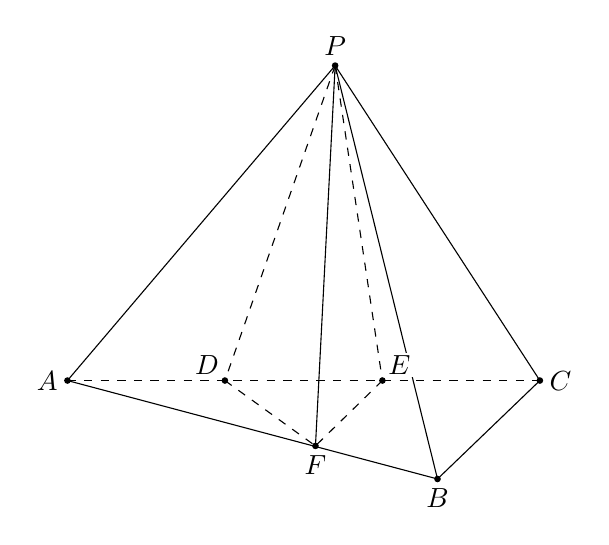
\begin{tikzpicture}[>=stealth,scale=1.0]
  % 顶点与底面各点
  \coordinate (P) at (3.4,4.0);
  \coordinate (A) at (0,0);
  \coordinate (C) at (6,0);
  \coordinate (B) at (4.7,-1.25);
  \coordinate (D) at (2,0);
  \coordinate (E) at (4,0);
  \coordinate (F) at (3.15,-0.83);
  % 实线棱
  \draw (P)--(A);
  \draw (P)--(B);
  \draw (P)--(C);
  \draw (P)--(F);
  \draw (A)--(B);
  \draw (B)--(C);
  % 虚线：AC 及内部线段
  \draw[dashed] (A)--(C);
  \draw[dashed] (P)--(D);
  \draw[dashed] (P)--(E);
  \draw[dashed] (D)--(F);
  \draw[dashed] (E)--(F);
  % 标号
  \fill (P) circle (1.2pt) node[above] {$P$};
  \fill (A) circle (1.2pt) node[left] {$A$};
  \fill (B) circle (1.2pt) node[below] {$B$};
  \fill (C) circle (1.2pt) node[right] {$C$};
  \fill (D) circle (1.2pt) node[fill=white,inner sep=1pt,above left=1pt] {$D$};
  \fill (E) circle (1.2pt) node[fill=white,inner sep=1pt,above right=1pt] {$E$};
  \fill (F) circle (1.2pt) node[below] {$F$};
\end{tikzpicture}
